\section{Development Process}
% - Methodology and stages of development
% - Challenges faced and solutions implemented

\subsection{Backend Development}
\subsubsection{Server and API Development}
% Design and implementation of the backend server.
% API functionalities for device and alert management.

% Development of an API for reloading Prometheus alert rules.
The backend server serves as the backbone and the controller of the acoustic event classification demonstration system. It is designed with a focus on handling user data management requests, ensuring responsiveness of database manipulation, and maintaining robust communication with various system components. The server is developed using \textsc{Node.js}, chosen for its performance efficiency and scalability.

The API facilitates seamless interaction between the frontend application, the classification model, and the database. The development of the API followed RESTful principles to ensure standardization and ease of integration. Key functionalities include:

\begin{itemize}
  \item \textbf{Device Management}: This endpoint allows for registering, updating, and removing devices involved in acoustic event detection. It is important to enable dynamic management of devices given the scalable nature of the application.
  \item \textbf{Alert Management}: This functionality provides endpoints to configure, update, and delete alert conditions. Alerts are triggered based on specific acoustic event classifications, and this API endpoint allows users to customize their alert parameters.
  \item \textbf{Reloading Prometheus Alert Rules}: To ensure real-time monitoring and alerting, an API endpoint is created for reloading \textsc{Prometheus} alert rules. This feature allows for immediate updates in the monitoring system without requiring a server restart, thereby enhancing the system’s efficiency and uptime.
\end{itemize}

According to the requirements, the API scheme is designed as in \ref{table:api}.

\begin{table}[h!]
  \centering
  \begin{tabular}{|l|c|l|}
    \hline
    Endpoint                          & Method & Description                                                                                              \\ [0.5ex]
    \hline\hline
    \texttt{\lstinline{/api/devices}} & GET    & Retrieve a list of devices                                                                               \\
    \hline
    \texttt{\lstinline{/api/devices/:deviceId}}    & GET    & Retrieve information of the Device with \texttt{\lstinline{deviceId}}                       \\
    \hline
    \texttt{\lstinline{/api/devices/:deviceId}} & POST   &   Update information of the Device with \texttt{\lstinline{deviceId}}                          \\
    \hline
    \texttt{\lstinline{/api/devices/:deviceId}} & PUT    &    Add a Device with \texttt{\lstinline{deviceId}}                                             \\
    \hline
    \texttt{\lstinline{/api/devices/:deviceId}} & DELETE &    Delete the Device with \texttt{\lstinline{deviceId}}                                        \\
    \hline
    \texttt{\lstinline{/api/alerts}}  & GET    & Retrieve a list of alerts                                                                                \\
    \hline
    \texttt{\lstinline{/api/alerts/:alertId}}    & GET    & Retrieve information of the Alert with \texttt{\lstinline{alertId}}                           \\
    \hline
    \texttt{\lstinline{/api/alerts/:alertId}} & POST   &   Update information of Alert with \texttt{\lstinline{alertId}}                                  \\
    \hline
    \texttt{\lstinline{/api/alerts/:alertId}} & PUT    &    Add an Alert with \texttt{\lstinline{alertId}}                                                \\
    \hline
    \texttt{\lstinline{/api/alerts/:alertId}} & DELETE &    Delete the Alert with \texttt{\lstinline{alertId}}                                            \\
    \hline
    \texttt{\lstinline{/api/reload}} & POST &                                                                      Reload \textsc{Prometheus} Alert rules \\ [1ex]
    \hline
  \end{tabular}
  \caption{\label{table:api}RESTful API Endpoints}
\end{table}


The API is developed iteratively, beginning with defining the schema and endpoints. Following best practices, each endpoint is thoroughly tested for performance and security. Special attention is given to:

\begin{itemize}
  \item \textbf{Security}: Implementing authentication and authorization mechanisms to secure access to the API.
  \item \textbf{Error Handling}: Robust error handling is implemented to ensure the API provides clear, useful feedback for any invalid requests or system failures.
  \item \textbf{Documentation}: Comprehensive documentation is created for the API, making it easier for front-end developers and future contributors to understand and utilize the API effectively.
\end{itemize}

The server and API development phase is critical in establishing a robust foundation for the acoustic event classification demonstration system. Through a combination of careful planning, strategic use of technology, and rigorous testing, a scalable and efficient backend infrastructure is successfully implemented.

\subsubsection{MQTT-Exporter Implementation}
% Implementation of MQTT-exporter to record classifier results.
% Process of exposing these results to Prometheus in the Prometheus metric format.

In the development of the MQTT-Exporter, a key component is establishing a reliable method for capturing and processing data from various devices. The MQTT-Exporter plays a crucial role in bridging the gap between the raw data emitted by the acoustic event classifiers and the \textsc{Prometheus} monitoring system. The implementation process can be broken down into several steps:

\begin{itemize}
  \item \textbf{Subscription to MQTT Topics}: \begin{itemize}
          \item \textbf{Topic Subscription}: The MQTT-Exporter is configured to subscribe to a wildcard topic, effectively enabling it to listen to all messages across multiple device topics. This approach ensured comprehensive data capture, as it allowed the exporter to receive data from an array of devices without needing individual subscriptions for each.
          \item \textbf{Data Capture Strategy}: Upon receiving data, the MQTT-Exporter parses and processes the messages. Given the diversity of data from various devices, the implementation includes robust error handling and data validation to ensure accuracy and consistency in the data being forwarded to \textsc{Prometheus}.
        \end{itemize}
  \item \textbf{Data Processing and Formatting}: \begin{itemize}
          \item \textbf{Message Processing}: Each MQTT message contains key information about acoustic events, such as event type, timestamp, and device ID. The processing logic extracts these details, transforming the raw data into a structured format suitable for \textsc{Prometheus}.
          \item \textbf{Metric Conversion}: The structured data is then converted into \textsc{Prometheus} metrics. This step involves mapping the extracted information to \textsc{Prometheus}'s data model, ensuring that each piece of data is correctly labeled and formatted as per \textsc{Prometheus} standards.
        \end{itemize}
  \item \textbf{Serving HTTP Requests from Prometheus}: \begin{itemize}
          \item \textbf{HTTP Endpoint Creation}: The MQTT-Exporter is equipped with an HTTP server to expose the collected metrics. This server acts as an endpoint for \textsc{prometheus} to scrape data.
          \item \textbf{Prometheus Scrape Configuration}: Within \textsc{Prometheus}, the scrape configuration is adjusted to include the MQTT-Exporter's HTTP endpoint. This setup ensures that \textsc{Prometheus} could regularly pull the latest data from the exporter.
          \item \textbf{Security and Reliability}: Additional considerations are given to secure this HTTP communication and to ensure the reliability and uptime of the MQTT-Exporter service, as it is a critical link in the data pipeline.
        \end{itemize}
  \item \textbf{Integration Testing and Optimization}: \begin{itemize}
          \item \textbf{Testing with Multiple Devices}: Rigorous testing is conducted to ensure that the MQTT-Exporter can handle data from a wide range of devices concurrently, without any loss in data integrity or system performance.
          \item \textbf{Performance Optimization}: Based on the testing outcomes, several optimizations are made to enhance the efficiency of the MQTT-Exporter, such as optimizing the message parsing logic and improving the data handling capacity of the HTTP server.
        \end{itemize}
\end{itemize}

This MQTT-Exporter implementation is a pivotal part of the system, enabling seamless and efficient communication between the distributed device data sources and the centralized \textsc{Prometheus} monitoring system. Through this integration, real-time monitoring and analysis of acoustic event classification become possible, greatly enhancing the system's overall capabilities.

\subsection{Infrastructure Setup}
\subsubsection{\textsc{Docker Compose} Environment}
% Configuration and deployment using Docker Compose.
In this project, \textsc{Docker Compose} is employed to define and run multi-container \textsc{Docker} applications. The primary motivation for using \textsc{Docker Compose} is to ensure a consistent and isolated environment across different development and deployment stages. The \textsc{Docker Compose} files are configured to orchestrate various services such as the backend server, \textsc{Eclipse Mosquitto}, \textsc{Prometheus}, \textsc{Grafana}, \textsc{Alertmanager}, \textsc{Nginx}, and \textsc{Traefik} proxy. This approach significantly streamlines the deployment process and allows for easy scalability and maintenance.

With the help of \textsc{Docker} Networks, we deploy the whole project under an independent subnet, which limits the access to our backend components, and isolates and protects the backend services.

\subsubsection{\textsc{Eclipse Mosquitto} Setup}
% Implementation of file-based user and ACL management.
% Integration of Mosquitto-exporter with \textsc{Prometheus}.
We set up \textsc{Eclipse Mosquitto}, an open-source message broker that implements the MQTT protocol, for handling real-time data communication. Particular attention is paid to security and management. User authentication is managed through password files, providing a simple yet effective way to control access. Access Control Lists (ACLs) are used to grant specific permissions to different users, ensuring secure and restricted access to topics. We also deploy \textsc{mosquitto-exporter}\cite{mosquittoexporter} which is integrated with \textsc{Prometheus} to expose message broker metrics, aiding in the monitoring and performance analysis of the MQTT broker.

\subsubsection{\textsc{Prometheus} Configuration}
% Details on setting up Prometheus with specific parameters.
\textsc{Prometheus} is chosen for its powerful monitoring capabilities and its suitability for dynamic, cloud-based environments. The \texttt{\lstinline{--web.enable-lifecycle}} flag is used to enable dynamic configuration reloading, allowing updates to the monitoring configuration without restarting the service.

\textsc{Prometheus} is configured to scrape \textsc{Prometheus} itself, \textsc{Grafana}, \textsc{mosquitto-exporter} and the MQTT-exporter we developped.

\subsubsection{\textsc{Grafana} Dashboard Development}
% Process of provisioning Grafana dashboards.
% Design and development of various dashboard views.
\textsc{Grafana} is utilized for its advanced data visualization capabilities. As in figure \ref{fig:grafana} Several custom dashboard views are developed, including heatmaps and calendar views, to effectively represent the acoustic event classification data. Dashboards are provisioned so that they are pre-configured as part of the setup, ensuring immediate availability upon deployment. We configure \textsc{Grafana} to support embedding, enabling the integration of visualizations into other components in our system.

\begin{figure}[htbp]
  \centering
  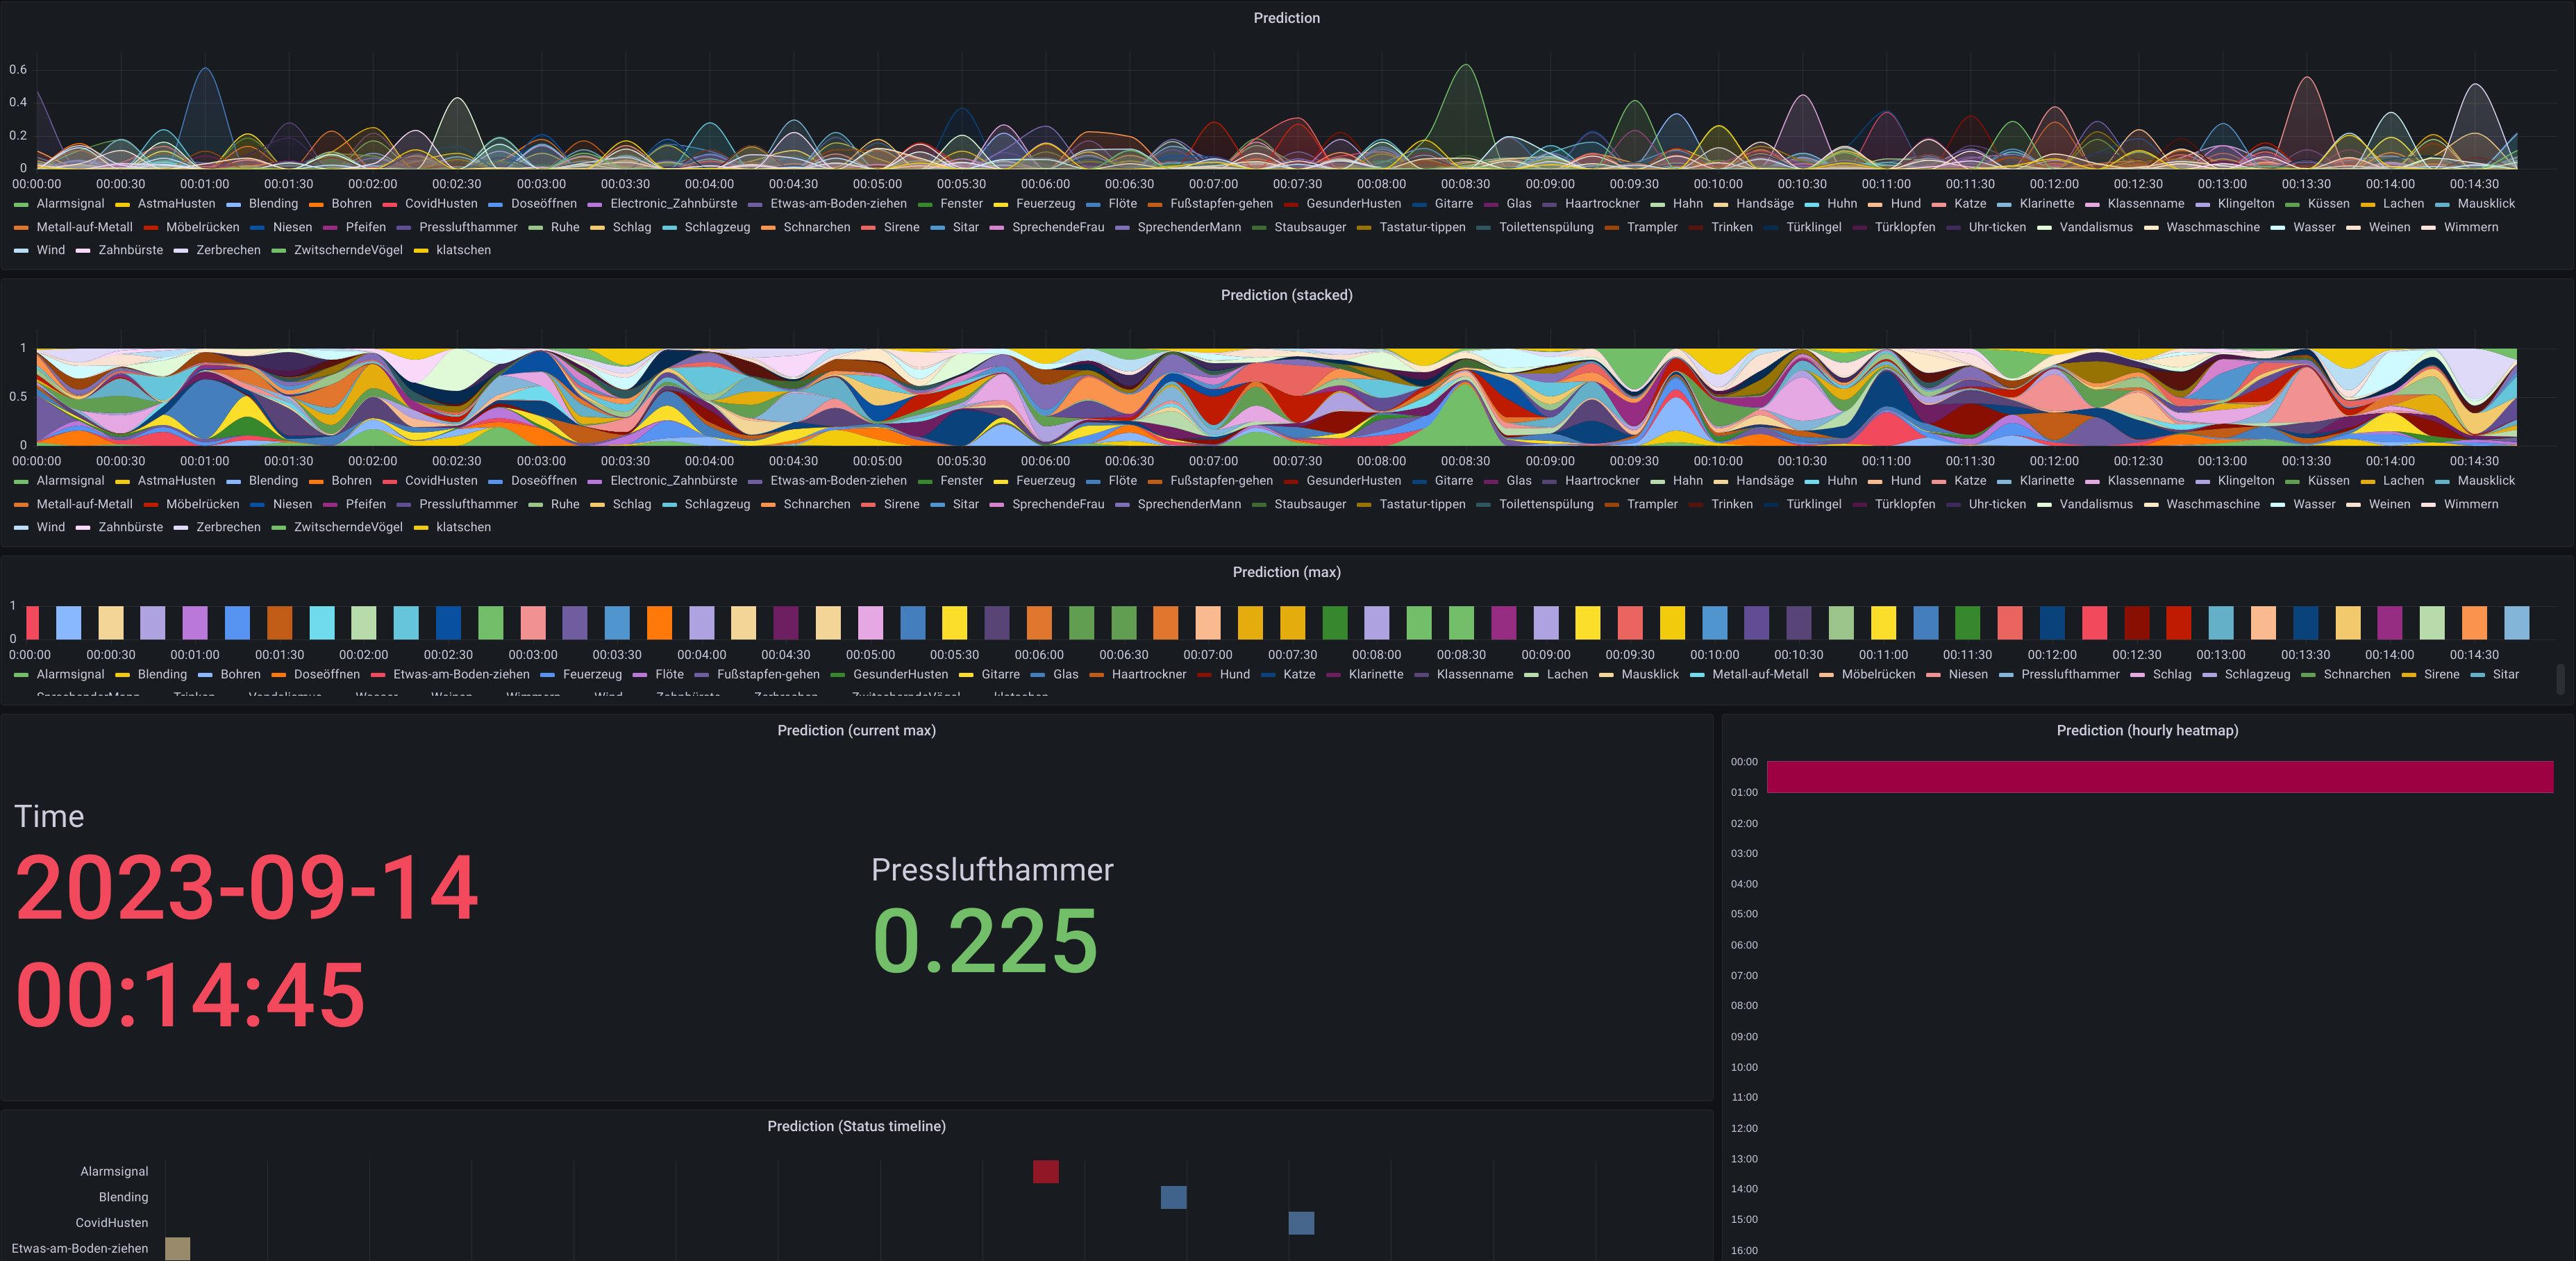
\includegraphics[width=0.85\textwidth]{Pictures/grafana}
  \caption{\label{fig:grafana}Grafana Dashboards}
\end{figure}

\subsubsection{\textsc{Alertmanager} Configuration}
% Setup and configuration of email alerts.
\textsc{Alertmanager} is integrated to handle alerts generated by \textsc{Prometheus}. A robust email notification system is set up, allowing for immediate alerting on predefined conditions.

\subsubsection{\textsc{Nginx} HTTP Server}
% Utilization of Nginx for serving static frontend builds.
\textsc{Nginx} is deployed to serve static frontend builds, ensuring fast and secure delivery of our frontend assets.

\subsubsection{\textsc{Traefik} Proxy}
% Configuration of Traefik proxy for domain name management and CSRF prevention.
\textsc{Traefik} is configured to enable the use of a single domain name for different services (frontend, backend API, MQTT), addressing same-origin requests problem. Integrated with \textsc{Cloudflare} and \textsc{LetsEncrypt}, \textsc{Traefik} also provides HTTPS support, enhancing the security of the system.

The overall Infrastructure is shown in \ref{fig:infra}.

\begin{figure}[htbp]
  \centering
  \begin{tikzpicture}[node distance=1cm, thick,
      block/.style={rectangle, draw, text width=6em, text centered, minimum height=4em}]

    % Nodes
    \node[block] (traefik) {Traefik};
    \node[block, below=of traefik] (nginx) {Nginx};
    \node[block, left=of nginx] (nodejs) {Node.js Backend};
    \node[block, right=of nginx] (mosquitto) {Mosquitto MQTT Broker};
    \node[block, right=of mosquitto] (mqttexporter) {MQTT-Exporter};
    \node[block, below=of mosquitto] (prometheus) {Prometheus};
    \node[block, below=of prometheus] (grafana) {Grafana};
    \node[block, above=of mqttexporter] (classifier) {Acoustic Event Classifier};

    % Connections
    \draw[->] (traefik) -- (nginx);
    \draw[->] (traefik) -- (nodejs);
    \draw[->] (traefik) -- (mosquitto);
    \draw[->] (nodejs) -- (prometheus);
    \draw[->] (mosquitto) -- (mqttexporter);
    \draw[->] (mqttexporter) -- (prometheus);
    \draw[->] (prometheus) -- (grafana);
    \draw[->] (classifier) -- (mosquitto);

  \end{tikzpicture}
  \caption{\label{fig:infra}Infrastructure}
\end{figure}

\subsection{Frontend Development}
\subsubsection{Framework and Styling}
% Choice of ReactJS and React-Router for the frontend framework.
% Use of Bootstrap v5 for styling and accessibility considerations.
% Application of D3.js for data visualization.

We choose \textsc{React.js} for its efficiency in rendering and updating components dynamically, essential for handling live data streaming. \textsc{react-router} is integrated using the \texttt{\lstinline{BrowserRouter}} for its compatibility and ease of creating a navigable single-page application. This approach allows us to create a seamless user experience without full page reloads. Routes are meticulously designed to facilitate easy navigation and logical access to different functionalities of the application. The structure of these routes includes:

\begin{itemize}
  \item \texttt{\lstinline{/live}} and \texttt{\lstinline{/live/:deviceId}} for accessing live data streams.
  \item \texttt{\lstinline{/device}} and \texttt{\lstinline{/device/:deviceId}} for device management.
  \item \texttt{\lstinline{/alert}} and \texttt{\lstinline{/alert/:alertId}} for alert management.
  \item \texttt{\lstinline{/query}} and \texttt{\lstinline{/query/:visualizationType}} for querying and visualizing historical data.
  \item \texttt{\lstinline{/settings}} for configuration settings.
  \item \texttt{\lstinline{/logout}} for user logout functionality.
\end{itemize}

We select Bootstrap v5 as our basic design system. It provides a robust foundation for styling basic elements and we use it to ensure a responsive layout across various devices and screen sizes. We leverage Bootstrap's grid system to establish the basic layout of the application, ensuring that each component and page is both aesthetically pleasing and functional. We give special attention to making the interface accessible, aligning with Bootstrap’s accessibility features.

For the data visualization aspect of our frontend, we choose \textsc{D3.js} library to create complex and interactive visualizations, which is a core requirement for representing the classifier’s real-time data. We utilize \textsc{D3.js} to implement a dynamic heatmap visualization, which presents the classification results in an understandable and insightful manner.

The integration of D3.js with \textsc{React.js} posed certain challenges due to their differing approaches to DOM manipulation. To overcome this, we develop custom hooks in \textsc{React.js} to encapsulate \textsc{D3.js} code, ensuring that the \textsc{D3.js} visualizations were seamlessly integrated into the \textsc{React.js} component lifecycle. This approach maintains \textsc{React.js}'s declarative nature while leveraging \textsc{D3.js}'s powerful data-driven transformation capabilities.

\subsubsection{Single Page Web Application Development}
% Development process of the single page application.
% Integration with the MQTT server for live data streaming.

We utilize \textsc{mqtt.js} to establish a reliable connection for live data streaming from the acoustic event classifier. This allows for the real-time reception of data on the frontend. \textsc{D3.js} is employed to render this data stream into an intuitive and interactive heatmap. The visualization represents the last 60 seconds of data on the x-axis, with classification tags on the y-axis. The color intensity in the heatmap corresponds to the confidence level of each prediction. We face challenges in synchronizing the high-velocity data stream with the \textsc{D3.js} visualization. To address this, we implement efficient data-binding techniques and optimize the rendering process to ensure smooth, real-time updates.

We developed calendar heatmap components by embedding \textsc{Grafana} visualization plugins. This allows us to present historical data in a calendar format, providing users with an easy way to navigate and analyze past events. Special attention is paid to making this component user-friendly and visually appealing. We ensure that it is seamlessly integrated with the overall design of the web application.

User settings and preferences were stored in LocalStorage. This choice provided a simple and effective way to persist user-specific settings without the need for backend storage solutions.

We integrate \textsc{web-vitals} to collect key metrics like Cumulative Layout Shift (CLS), First Input Delay (FID), First Contentful Paint (FCP), Largest Contentful Paint (LCP), and Time to First Byte (TTFB). These metrics guide our optimization efforts during development. We use \textsc{stat.js} to display real-time performance metrics such as frames per second (FPS) and memory usage to users. This feature is particularly useful for monitoring the application's responsiveness and resource consumption.

To enhance user interaction, we implement a notification center using \textsc{react-toastify}. This allows us to display alerts and messages to users in a non-intrusive and user-friendly manner. The design and placement of notifications are carefully considered to ensure they are informative yet unobtrusive, enhancing the overall user experience.

\subsection{Technical Challenges and Solutions}
In this section, we will highlight some of the significant technical challenges encountered during the development of the acoustic event classification demonstration and the strategies employed to overcome these obstacles. This section aims to provide insights into problem-solving approaches and the application of technical knowledge in practical scenarios.


\subsubsection{Frontend Performance Optimization}
% Techniques used to optimize the performance of the system.
The core functionality of the system involves real-time processing and visualization of acoustic event classification data. This requires the system to handle continuous data streams efficiently and render visualizations with minimal latency. The challenge is to ensure that the live data stream from the MQTT server is processed and displayed in a heatmap format without significant delays, ensuring a seamless user experience.

To address this, \textsc{D3.js} transitions are used for dynamic data visualization. The rendering of each piece of data is called only once and the elements will be removed when they are outside the viewport of the visualization. This is to minimize unnecessary re-rendering, thus enhancing performance. With hooks of \textsc{React.js}, the side effects are well managed, and cleanups are done when the heatmap component is unmounted.

\subsubsection{User-Friendly and Accessible Design}
The system needs to be not only technically sound but also user-friendly and accessible to a diverse range of users. The challenge is to create an intuitive interface that caters to both technical and non-technical users.

User experience (UX) principles are carefully considered during the design phase. This involved creating intuitive navigation and clear, understandable visualizations. Bootstrap v5 is utilized for responsive design, ensuring that the application is accessible on various devices and screen sizes.
Feedback from initial user testing is incorporated to refine the UI/UX, ensuring that the system is easy to use and meets the needs of its users.

\subsubsection{Security Considerations}
% Security measures implemented throughout the development process.
With the system handling sensitive data and being accessible over the internet, ensuring security and data privacy is paramount. This includes protecting against common web vulnerabilities and securing data transmission.

Security measures such as HTTPS support with Cloudflare and Let's Encrypt are carried out to encrypt data in transit. \textsc{Mosquitto’s} file-based user and ACL management are used to control access and ensure that users can access only what they are authorized to. Regular security audits are conducted, and industry-standard security practices like OWASP Application Security Verification Standard (ASVS) are followed to protect against common web vulnerabilities like CSRF, XSS, and SQL injection.

\subsection{Project Management and Development Practices}
% If applicable, detail the use of Agile methodologies in project management.
% Utilization of version control systems and collaborative tools.
In the development of the acoustic event classification demonstration, project management and development practices are carried out to ensure an organized and efficient workflow. Central to these practices is the use of GitHub for issue tracking and version control.

\subsubsection{Issue Tracking with GitHub}
The project leveraged GitHub's issue-tracking system to organize tasks, bugs, and feature requests. Each issue is clearly defined with labels for easy categorization and prioritization. Milestones are created on GitHub to group issues into manageable phases, aligning with specific development goals and timelines. This helps in maintaining a clear vision of the project roadmap and deadlines. The progress of each issue is regularly updated, providing transparency and allowing for real-time tracking of the project's advancement.

\subsubsection{Version Control and Collaboration}
A structured branching strategy is employed, with separate branches for features, hotfixes, and releases. This approach ensures that the development of new features does not disrupt the main codebase. Automated build and test processes are integrated into the GitHub repository, ensuring that each commit and merge request adheres to the project's quality standards.